\setlength{\footskip}{8mm}

\chapter{Extracting the Object from the Shadows: Maximum Likelihood
Object/Shadow Discrimination}
\label{ch:shadow}

\textit{In this chapter, we propose and experimentally evaluate a new
method for detecting shadows using a simple maximum likelihood
formulation based on color information. We first estimate, offline, a
joint probability distribution over the difference in the HSV color
space between pixels in the current frame and the corresponding pixels
in a background model, conditional on whether the pixel is an object
pixel or a shadow pixel.  Given the learned distribution, at run time,
we use the maximum likelihood principle to classify each foreground
pixel as either shadow or object.  In an experimental evaluation, we
find that the method outperforms standard methods on three different
real-world video surveillance data sets.  We conclude that the
proposed shadow detection method would be an extremely effective
component in an intelligent video surveillance system.}

\section{Introduction}

In many video surveillance applications, detecting and tracking moving
objects is an important issue. A \DIFdelbegin \DIFdel{very }\DIFdelend common approach to detect moving
objects is to apply background a subtraction algorithm. However,
background subtraction algorithms share one major disadvantage:
shadows tend to be misclassified as part of the foreground
object. This can lead to many undesirable consequences in the
detection step while segmenting and extracting features of moving
objects. For example, any estimate of the size of the detected object
would be an overestimate due to the misclassification of shadow pixels
as foreground pixels. Additionally, during object segmentation,
shadows misclassified as moving objects could lead to merging
otherwise separate blobs representing different people walking close
to each other.  This would make isolating and tracking people in a
group much more difficult than necessary.

Since shadow removal can significantly improve the performance of
computer vision tasks such as tracking, segmentation, and object
detection, shadow detection has become an active research area in
recent years.

Several well-known algorithms for shadow detection already exist. Most
of the work is based on background modeling and color difference
information. Generally, some model of the background is estimated,
then the difference between the background and current image is used
to identify changed pixels, then the changed pixels are further
classified into object and shadow.  Shadow pixels tend to have similar
chromaticity but lower luminance than the corresponding background
pixel.  In the RGB color space, chromaticity and luminance are not
orthogonal, but lighting differences can be controlled for in the
normalized RGB color space \shortcite{finlayson98colour}.  Some
research work thus utilizes the normalized RGB space in the background
subtraction and shadow removal
algorithm \shortcite{mckenna00tracking,elgammal02background,hong03background}.

\shortciteA{mikic00shadow} observe that in the normalized RGB color
space, shadow pixels tend to be more blue and less red than
illuminated pixels.  They apply a probabilistic model based on the
normalized red and blue features to classify shadow pixels in traffic
scenes. The authors assume that the background and shadow values
follow Gaussian distributions and foreground values follow a uniform
distribution. They iteratively estimate the posterior probabilities of
a given pixel belonging to each of three classes: background, shadow,
and foreground, until one of the probabilities reaches a fixed
threshold. The pixel is then classified accordingly.  If none of the
three probabilities reaches the threshold, the pixel is classified as
background.

\shortciteA{salvador04shadow} propose a new method for detecting
cast shadows. They first identify the presence of shadows in the RGB
color space based on the fact that shadows darken the surface they
cast on. The detected regions are further verified based on the color
invariance and geometric properties expected of shadows.

\shortciteA{havasi06geometric} illustrate that color-based methods
work well for weak shadows but not strong shadows. Hence, they
integrate geometric information into the detection process, resulting
in an iterative Bayesian framework combining both color and geometric
information that improves detection results.

One well-known problem with the normalized RGB space is that
normalization of pixels with low intensity results in unstable
chromatic
components \shortcite{kender76color}. \shortciteA{cucchiara01shadow}
and \shortciteA{chen08shadow} propose a HSV color-based method to
distinguish shadows from moving objects that eliminates this
concern. Their approach is based on the assumption that only the
intensity of the area covered by shadows will significantly
change. Therefore, they detect shadows using the so-called
deterministic nonmodel-based (DNM) approach as follows:
\[
  SP_t (x,y) = \left\{ 
  \begin{array}{ll}
    1 & {\rm if} \; \alpha \le \frac{{I_t^V (x,y)}}{{B_t^V (x,y)}} \le \beta\\ 
    & \;\;\; \wedge \; (I_t^S (x,y) - B_t^S (x,y)) \le T_S  \\ 
    & \;\;\; \wedge \left| {I_t^H (x,y) - B_t^H (x,y)} \right| \le T_H\\ \\
    0 & {\rm otherwise}, \\ 
  \end{array} \right.
\]
where $SP_t(x,y)$ is the resulting binary mask for shadows at each
pixel $(x,y)$ at time $t$.  $I_t^H$, $I_t^S$, $I_t^V$, $B_t^H$,
$B_t^S$, and $B_t^V$ are the H, S, and V components of foreground
pixel $I_t(x,y)$ and background pixel $B_t(x, y)$ at pixel $(x,y)$ at
time $t$, respectively.  They prevent foreground pixels from being
classified as shadow pixels by setting two thresholds, $0 < \alpha <
\beta < 1$.  The four thresholds $\alpha$, $\beta$, $T_S$, and $T_H$
are empirically determined.

Some researchers have investigated color spaces besides RGB and
HSV. \shortciteA{blau06shadow} use an ``improved'' hue, luminance, and
saturation (IHLS) color space for shadow detection to deal with the
issue of unstable hue at low saturation by modeling the relationship
between them. They then perform simple background subtraction method
based on the IHLS color space and saturation-weighted hue statistics.
Their experimental results show that detecting shadows in this color
is more reliable than in normalized RGB or HSV color spaces in several
video sequences.

Another alternative color space is YUV.  Some applications such as
television and videoconferencing use the YUV color space natively, and
since transformation from YUV to HSV is
time-consuming, \shortciteA{schreer02shadow} operate in the YUV color
space directly, developing a fast shadow detection algorithm based on
approximated changes of hue and saturation in the YUV color space.

There has been some work using texture-based methods such as the
normalized cross-correlation (NCC)
technique \shortcite{tian05shadow,jacques05shadow}. This method
detects shadows based on the assumption that the intensity of shadows
is proportional to the incident light, so shadow pixels should simply
be darker than the corresponding background pixels. Under this
assumption, shadow patches should be scaled versions of the
corresponding background patches. This assumption is most valid in
scenes with visible background texture inside the shadows. The method
computes the NCC between the neighborhood of a pixel in the foreground
mask and the neighborhood of the corresponding pixel in the background
model.  For each pixel $(i, j)$ of the foreground mask, it considers a
$(2N + 1)
\times (2N + 1)$ template $T_{ij}$ defined by $T_{ij}(n, m) = I(i+n,
j+m)$ for $-N \le n \le N$ and $-N \le m \le N$ ($N$ is empirically
determined). If $B(i, j)$ is the background model, the NCC value at
pixel $(i, j)$ is defined as follows:
\[
  NCC(i,j) = \frac{{ER(i,j)}}{{E_B (i,j)E_{T_{ij} } }},
\]
where
\[
  ER(i,j) = \sum\limits_{n = -N}^N {\sum\limits_{m = -N}^N {B(i + n,j
  + m)T_{ij} (n,m)}},
\]
\[
  E_B (i,j) = \sqrt {\sum\limits_{n = -N}^N {\sum\limits_{m = -N}^N
  {B(i + n,j + m)^2}}},
\]
\[
  E_{T_{ij} } = \sqrt {\sum\limits_{n = -N}^N {\sum\limits_{m = -N}^N
  {T_{ij} (n,m)^2}}}.
\]
For a pixel in a shadow region, the NCC value should be large (close
to one) and the $E_{T_{ij}}$ for the region around $(i,j)$, i.e., its
magnitude, should be smaller than $E_B (i,j)$. Consequently, a pixel
is classified as shadow if
\[
  NCC(i,j) \ge L_{NCC} 
\]
and
\[
  E_{T_{ij}} < E_B (i,j),
\]
where $L_{NCC}$ is an empirical threshold.

However, the texture-based method tends to misclassify foreground
pixels as shadow pixels when the foreground region has a similar
texture to the corresponding background
region. \shortciteA{xu05shadow} propose a hybrid shadow removal
technique that combines color and texture-based procedures to detect
shadows.  Since chromaticity in a shadow region should be the same as
the corresponding background region, and since the texture in a shadow
region should be the same as the corresponding background region, the
authors first classify pixels based on a set of thresholds for
brightness and color distortion then perform speckle removal filtering
to reconstruct the final foreground shapes.

Here we propose a new method for detecting shadows using maximum
likelihood estimation based on color information.  We extend the
deterministic nonmodel-based approach to parametric statistical
model-based approach. Our method estimates the joint distribution over
the difference in the HSV color space between pixels in the current
frame and the corresponding pixels in a background model, conditional
on whether the pixel is an object pixel or a shadow pixel. At run
time, we simply use the maximum likelihood principle to classify each
foreground pixel as either shadow or object given the estimated model.
Experimental results demonstrate that our proposed method outperforms
the standard methods (DNM and NCC) on three different real-world video
surveillance data sets. Our method is thus effective and also has the
potential to improve the object detection and motion analysis module
in intelligent video surveillance systems.

In the rest of this chapter, I provide details of the proposed method
and the overall process in Section \ref{sec:shadow-algorithm},
demonstrate the effectiveness of the shadow detection method with an
experimental evaluation in Section \ref{sec:shadow-results}, and then
conclude and point to future work in
Section \ref{sec:shadow-discussion}.

\section{Maximum Likelihood Classification of Foreground Pixels}
\label{sec:shadow-algorithm}

We divide our method into two phases.  In the first, offline phase, we
acquire training video, construct a background model from the first
few frames, perform foreground extraction on the remaining frames,
then manually label the extracted pixels as either object pixels or
shadow pixels.  I previously describe these steps in
Sections \ref{sec:blob-motion-detection}
and \ref{sec:blob-blob-extraction}. After that, we construct a joint
probability model over the difference in the HSV color space between
pixels in the current frame and the corresponding pixels in the
background model, conditional on whether the pixel is an object pixel
or a shadow pixel.

During the second, online phase, we perform the same background
modeling and foreground extraction procedure and further classify
foreground pixels as either shadow or object using the maximum
likelihood approach. I describe each of these steps in more detail in
the following sections.

\subsection{Offline Phase}

After foreground extraction, we manually label pixels as either shadow
or object. We then observe the distribution over the difference in hue
($H_{\text{diff}}$), saturation ($S_{\text{diff}}$), and value
($V_{\text{diff}}$) components in the HSV color space between pixels
in the current frame and the corresponding pixels in the background
model.  Figure \ref{fig:foreground-distribution} shows examples of
these distributions for object pixels, and
Figure \ref{fig:shadow-distribution} shows examples of these
distributions for shadow pixels.

\begin{figure}[t]
  \centering
  \subfloat[]{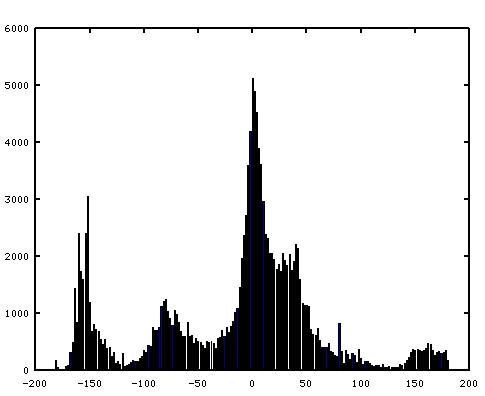
\includegraphics[scale=0.25]{figures/foreground_diff_h.png}}
  \hspace{0.05cm}
  \subfloat[]{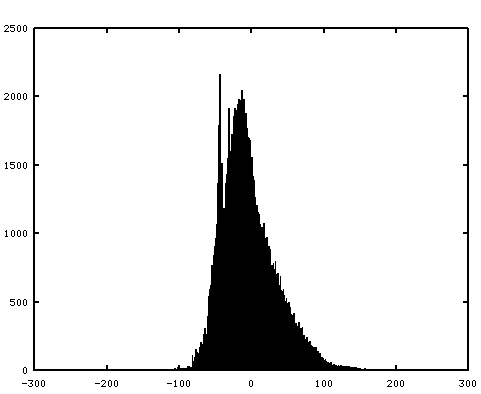
\includegraphics[scale=0.25]{figures/foreground_diff_s.png}}
  \hspace{0.05cm}
  \subfloat[]{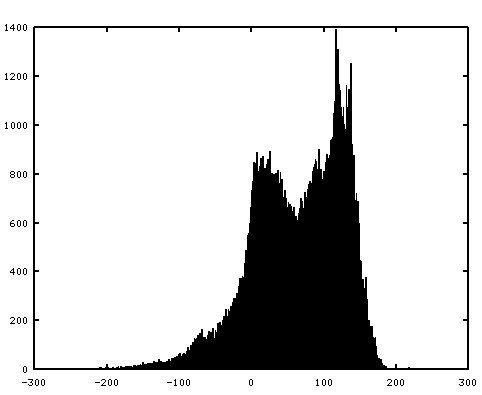
\includegraphics[scale=0.25]{figures/foreground_diff_v.png}}
  \caption[Example distributions over the difference in hue,
    saturation, and value components for true object pixels, extracted
    from our hallway dataset.]{\small Example distributions over the
    difference in (a) hue, (b) saturation, and (c) value components
    for true object pixels, extracted from our hallway dataset.}
  \label{fig:foreground-distribution}
\end{figure}

\begin{figure}[t]
  \centering
  \subfloat[]{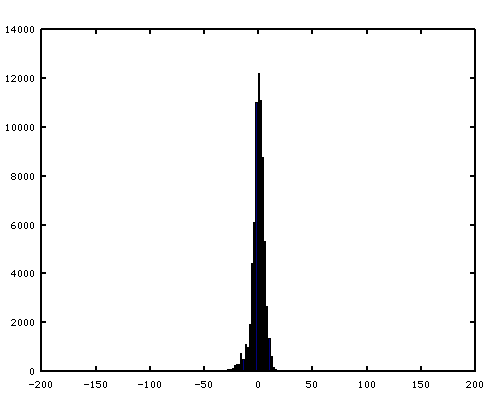
\includegraphics[scale=0.25]{figures/shadow_diff_h.png}}
  \hspace{0.05in}
  \subfloat[]{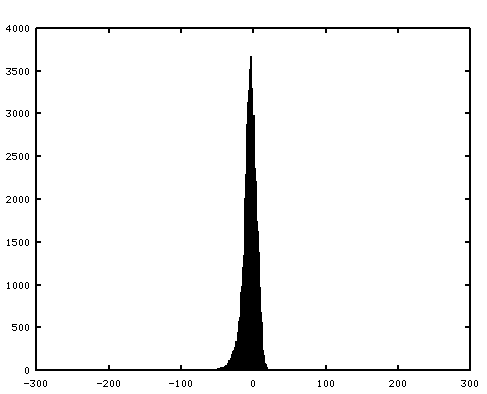
\includegraphics[scale=0.25]{figures/shadow_diff_s.png}}
  \hspace{0.05in}
  \subfloat[]{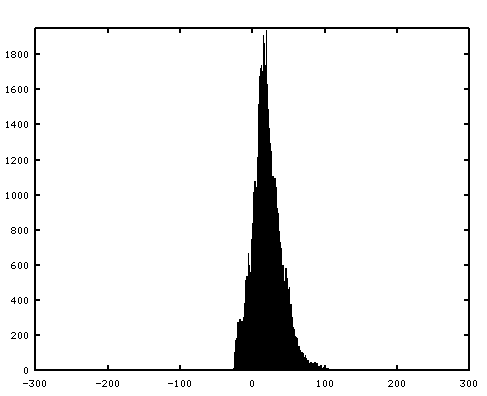
\includegraphics[scale=0.25]{figures/shadow_diff_v.png}}
  \caption[Example distributions over the difference in hue,
    saturation, and value components for true shadow pixels, extracted
    from our hallway dataset.]{\small Example distributions over the
    difference in (a) hue, (b) saturation, and (c) value components
    for true shadow pixels, extracted from our hallway dataset.}
  \label{fig:shadow-distribution}
\end{figure}

Clearly, in all three cases, the distributions for object pixels and
shadow pixels are very different.  We thus introduce a measurement
probability distribution conditional on whether the assignment for a
pixel is object or shadow. In this work, we assume that the individual
component difference distributions are conditionally independent given
the assignment.

We define the \DIFdelbegin \DIFdel{measurement likelihood }\DIFdelend \DIFaddbegin \DIFadd{probability of measurement }\DIFaddend for pixel $(x, y)$ given its 
assignment as follows.
\begin{equation}
  \label{eq:shadow-measurement}
  \begin{array}{ccl}
    P(M_{\text{xy}} \mid A_{\text{xy}} = \text{sh}) 
            & = & P(H_{\text{diff}} \mid A_{\text{xy}} = \text{sh}) \times \\
            &   & P(S_{\text{diff}} \mid A_{\text{xy}} = \text{sh}) \times \\
            &   & P(V_{\text{diff}} \mid A_{\text{xy}} = \text{sh}),
  \end{array}
\end{equation}
where $M_{xy}$ is a tuple containing the HSV value for pixel $(x,y)$
in the current image as well as the HSV value for pixel $(x,y)$ in the
background model for pixel $(x,y)$, and $A_{xy}$ is the assignment of
pixel $(x,y)$ as object or shadow. ``sh'' stands for shadow.

\DIFdelbegin \DIFdel{To make the problem tractable, we }\DIFdelend \DIFaddbegin \DIFadd{We }\DIFaddend assume that the distributions over the components on the right 
hand side in \ref{eq:shadow-measurement} 
follow Gaussian distributions, defined as follows.
\begin{equation*}
  P(H_{\text{diff}} \mid A_{\text{xy}} = \text{sh}) =
  {\cal N}(H_{\text{diff}} ;
  \mu_{h_{\text{diff}}^{\text{sh}}},
  \sigma^2_{h_{\text{diff}}^{\text{sh}}})
\end{equation*}
\begin{equation*}
  P(S_{\text{diff}} \mid A_{\text{xy}} = \text{sh}) =
  {\cal N}(S_{\text{diff}} ;
  \mu_{s_{\text{diff}}^{\text{sh}}},
  \sigma^2_{s_{\text{diff}}^{\text{sh}}})
\end{equation*}
\begin{equation*}
  P(V_{\text{diff}} \mid A_{\text{xy}} = \text{sh}) =
  {\cal N}(V_{\text{diff}} ;
  \mu_{v_{\text{diff}}^{\text{sh}}},
  \sigma^2_{v_{\text{diff}}^{\text{sh}}})
\end{equation*}
\DIFaddbegin \DIFadd{Although the distributions for the true object pixels are clearly 
non-Gaussian as seen in Figure~\ref{fig:foreground-distribution}, 
I plan to extend this chapter in future work, but in 
this version, I simply use the sample mean and variance. However, 
on extension of the work, we will definitely investigate better 
estimators and different distributions.
}

\DIFaddend Similarly, the \DIFdelbegin \DIFdel{measurement likelihood }\DIFdelend \DIFaddbegin \DIFadd{probability of measurement given its assignment }\DIFaddend for 
object pixels can be computed as follows.
\begin{equation}
  \label{eq:foreground-measurement}
  \begin{array}{ccl}
    P(M_{\text{xy}} \mid A_{\text{xy}} = \text{obj}) 
            & = & P(H_{\text{diff}} \mid A_{\text{xy}} = \text{obj}) \times \\
            &   & P(S_{\text{diff}} \mid A_{\text{xy}} = \text{obj}) \times \\
            &   & P(V_{\text{diff}} \mid A_{\text{xy}} = \text{obj})
  \end{array}
\end{equation}
Here ``obj'' stands for object. As for the shadow pixel distributions,
we assume Gaussian distributions over the components on the right hand
side in \ref{eq:foreground-measurement}, as follows.
\begin{equation*}
  P(H_{\text{diff}} \mid A_{\text{xy}} = \text{obj}) =
  {\cal N}(H_{\text{diff}} ;
  \mu_{h_{\text{diff}}^{\text{obj}}},
  \sigma^2_{h_{\text{diff}}^{\text{obj}}})
\end{equation*}
\begin{equation*}
  P(S_{\text{diff}} \mid A_{\text{xy}} = \text{obj}) =
  {\cal N}(S_{\text{diff}} ;
  \mu_{s_{\text{diff}}^{\text{obj}}},
  \sigma^2_{s_{\text{diff}}^{\text{obj}}})
\end{equation*}
\begin{equation*}
  P(V_{\text{diff}} \mid A_{\text{xy}} = \text{obj}) =
  {\cal N}(V_{\text{diff}} ;
  \mu_{v_{\text{diff}}^{\text{obj}}},
  \sigma^2_{v_{\text{diff}}^{\text{obj}}})
\end{equation*}
We estimate the parameters $\Theta = \{
\mu_{h_{\text{diff}}^{\text{sh}}},
\sigma^2_{h_{\text{diff}}^{\text{sh}}},
\mu_{s_{\text{diff}}^{\text{sh}}},
\sigma^2_{s_{\text{diff}}^{\text{sh}}},
\mu_{v_{\text{diff}}^{\text{sh}}},
\sigma^2_{v_{\text{diff}}^{\text{sh}}},
\mu_{h_{\text{diff}}^{\text{obj}}},
\sigma^2_{h_{\text{diff}}^{\text{obj}}},
\mu_{s_{\text{diff}}^{\text{obj}}},
\sigma^2_{s_{\text{diff}}^{\text{obj}}},
\mu_{v_{\text{diff}}^{\text{obj}}},
\sigma^2_{v_{\text{diff}}^{\text{obj}}} \}$ directly from training
data during the offline phase.

\subsection{Online Phase}

Given the model estimate $\Theta$, we use the maximum likelihood
approach to classify a pixel as a shadow pixel if
\begin{equation}
  \label{eq:ml}
  P(M_{\text{xy}} \mid A_{xy}=\text{sh} ; \Theta ) >
  P(M_{\text{xy}} \mid A_{xy}=\text{obj} ; \Theta ).
\end{equation}
Otherwise, we classify the pixel as an object pixel.

We could add the prior probabilities to the shadow model and the
object model in \ref{eq:ml} to obtain a maximum a posteriori
classifier. In our experiments, we assume equal priors.

\section{Experimental Results}
\label{sec:shadow-results}

In this section, we present experimental results for our proposed
maximum likelihood (ML) classification method and compare the results
with two other methods from the literature, namely the deterministic
nonmodel-based (DNM)
method \shortcite{kender76color,cucchiara01shadow} and the normalized
cross-correlation (NCC)
method \shortcite{tian05shadow,jacques05shadow}.

\begin{figure}[t]
  \centering
  \subfloat[]{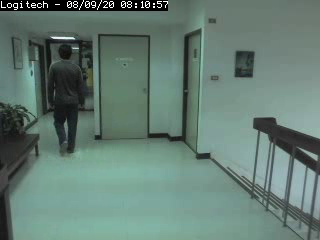
\includegraphics[scale=0.4]{figures/csim_hallway_benchmark.png}}
  \hspace{0.05cm}
  \subfloat[]{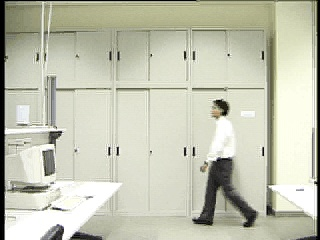
\includegraphics[scale=0.4]{figures/aton_lab_benchmark.png}}
  \hspace{0.05cm}
  \subfloat[]{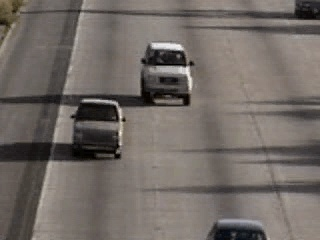
\includegraphics[scale=0.4]{figures/aton_highway1_benchmark.png}}
  \caption[Sample frames from the Hallway, Laboratory, and Highway
    video sequences.]{\small Sample frames from the (a) Hallway, (b)
    Laboratory, and (c) Highway video sequences}
  \label{fig:benchmark}
\end{figure}

We performed the experiments on three video sequences.
Figure \ref{fig:benchmark} shows sample frames from the three video
sequences. The video sequences include both indoor and outdoor
scenes. The \textit{Hallway} sequence\footnote{Freely available for
others to experiment with
at: \url{http://www.kanouivirach.com/#downloads}.} shows a hallway
scene. For this video, we mounted a CCTV camera to record in an
academic building. The \textit{Laboratory} sequence shows a laboratory
room, and the \textit{Highway} sequence shows a traffic scene. The
last two video sequences were first introduced in Prati et al.'s
work\nocite{prati03shadow}.

To evaluate the performance of the methods, we compute the two metrics
proposed by \shortciteA{prati03shadow}, defining the shadow detection
rate $\eta$ and the shadow discrimination rate $\xi$ as follows:
\[
  \eta = \frac{TP_{\text{sh}}}{TP_{\text{sh}} + FN_{\text{sh}}};\; 
  \xi = \frac{TP_{\text{obj}}}{TP_{\text{obj}} + FN_{\text{obj}}},
\]
where the subscript ``sh'' and ``obj'' stand for shadow and object,
respectively. $TP$ and $FN$ are the number of true positive (i.e., the
shadow or object pixels correctly identified) and false negative
(i.e., the shadow or object pixels classified incorrectly) pixels.
$\eta$ expresses the proportion of shadow pixels correctly detected,
and $\xi$ expresses the proportion of object pixels correctly
detected.  $\eta$ and $\xi$ can also be thought of as the true
positive rate (sensitivity) and true negative rate (specificity) for
detecting shadows, respectively. In the experiment, we also compare
the methods with the additional two metrics: precision and $F_1$
score.

\subsection{Preparation}

Ground truth data are provided with the \textit{Laboratory} and
\textit{Highway} video sequences in Sanin et al.'s work\nocite{sanin12shadow}. 
They used a standard Gaussian mixture (GMM) background
model\nocite{stauffer99background} to extract foreground pixels for
the two videos. They selected 20 frames including objects from
the \textit{Laboratory} sequence arbitrarily for labeling.  For
the \textit{Highway} sequence, they labeled one out of every twenty
frames including objects for a total of 20 frames.  For our
\textit{Hallway} video sequence, to prepare similar ground truth data,
we selected one out of every ten frames including objects for 20
frames and manually labeled each pixel of each frame as object,
background, or shadow. We used the previously mentioned extended
version of the GMM background model for foreground extraction, but the
results were not substantially different from those of the standard
GMM.

To find the best parameters for each model while avoiding overfitting,
for each of the three models and each of the three data sets, we
performed five-fold cross validation using 10 of the training frames,
reserving the remaining 10 frames for the final test. The 10 frames in
each case were the second of every two frames in sequential order. We
varied the parameter settings for each method on each video dataset
and selected the setting that maximized the $F_1$ score (a measure
combining both precision and recall) over the cross validation test
sets. Finally, we tested on the remaining 10-frame final test set for
each video sequence.

\subsection{Shadow Detection Performance}

Table \ref{tab:comparison-results} compares the shadow detection
results between the proposed, DNM, and NCC methods.  Our method
achieves the top performance for shadow detection rate $\eta$ and
$F_1$ score in every case. We also obtain a good shadow discrimination
rate $\xi$ and precision in all three video
datasets. Figure \ref{fig:results-for-arbitrary-frame} shows the
results for an arbitrary frame in each video sequence. Green pixels
are those labeled as object pixels and red pixels are those labeled as
shadow pixels. The results in the figure confirm that our proposed
method clearly outperforms the two standard methods in all three video
datasets.

\begin{table}[t]
  \caption[Comparison of shadow detection results between the
    proposed, DNM, and NCC methods.]{\small Comparison of shadow
    detection results between the proposed, DNM, and NCC methods.}
  \begin{center}
    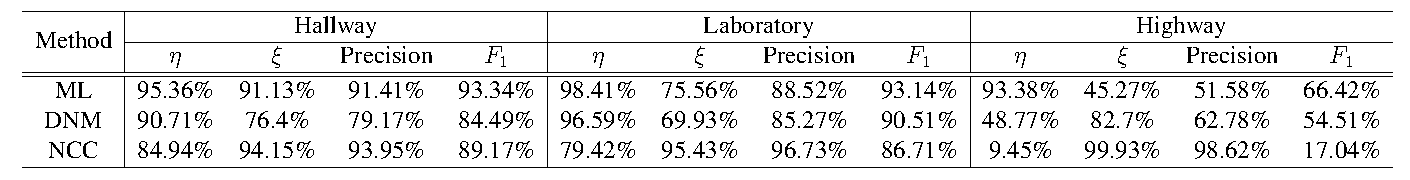
\includegraphics[width=6.1in]{figures/tab-shadow-results}
  \end{center}
  \label{tab:comparison-results}
\end{table}

\begin{figure}[t]
  \centering
  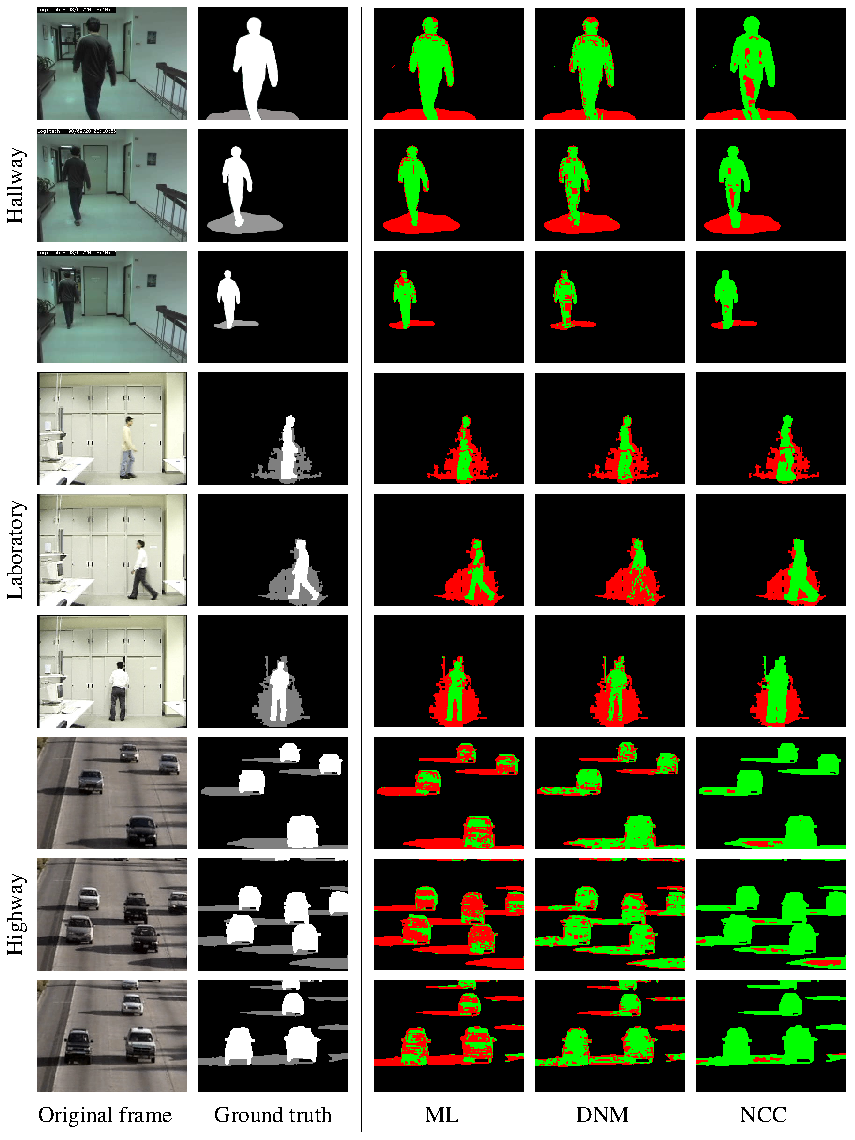
\includegraphics[width=6.2in]{figures/fig-shadow-results}
  \caption[Results for an arbitrary frame in each video
    sequence.]{\small Results for an arbitrary frame in each video
    sequence. The first column contains an example original frame for
    each video sequence. The second column shows the ground truth for
    that frame, where object pixels are labeled in white and shadow
    pixels are labeled in gray. The remaining columns show shadow
    detection results for each method, where pixels labeled as object
    shown in green and pixels labeled as shadow are shown in red.}
  \label{fig:results-for-arbitrary-frame}
\end{figure}

The DNM method has stable performance for all three videos, with good
performance for all metrics. Both the DNM method and our proposed
method suffer from the problem that the object colors can be confused
with the background color.  In the \textit{Highway} sequence (third
row in Figure \ref{fig:results-for-arbitrary-frame}), we clearly see
this situation. Our method detects shadows well but misclassifies some
object pixels as shadow, whereas DNM sometimes better discriminates
the shadow from the object.  However, the overall performance of our
proposed method is superior.

The NCC method achieves the best shadow discrimination rate $\xi$ and
precision. However, as can be seen in
Figure \ref{fig:results-for-arbitrary-frame}, this is because it
classifies nearly every pixel as object.  This gives NCC an advantage
for shadow precision and $\xi$ but on the other two metrics, shadow
detection rate $\eta$ and $F_1$ score, NCC performs extremely poorly
in all cases.  This is due to unclear background texture inside the
shadows, particularly on the \textit{Highway} sequence.

\section{Discussion}
\label{sec:shadow-discussion}

We propose a new method for detecting shadows using a simple maximum
likelihood approach based on color information.  We extend the
deterministic nonmodel-based approach, designing a parametric
statistical model-based approach. Our experimental results show that
our proposed method is extremely effective and superior to the
standard methods on three different real-world video surveillance data
sets.

In some cases, our method misdetects shadow pixels due to similar
color between the object and the background and unclear background
texture in shadow regions. Incorporating geometric or shadow region
shape priors would potentially improve the detection and
discrimination rates\DIFaddbegin \DIFadd{. 
}

\DIFadd{Additionally, the distributions over the difference 
in HSV color space for true object pixels and true shadow pixels remain 
static once trained. Therefore, the current approach may be inappropriate 
in the long run. More adaptive approach should be considered}\DIFaddend .

In future work, we plan to address these issues, further explore the
feasibility of combining our method with other useful shadow features,
and integrate our shadow detection module with a real-world open
source video surveillance system \shortcite{zoneminder}.

\FloatBarrier


%%% Old text %%%

%\section{Introduction}
%
%In video surveillance applications, moving object detection and
%tracking is an important issue.  A very common approach to detect
%moving objects is to apply a background subtraction technique. The
%process is basically to compare a new frame with a background
%model. The significant differences correspond to foreground. This
%process should ideally detect the moving objects and limit the false
%positive as much as possible at the same time.  More importantly, it
%should be able to avoid detection of shadows or noise. However, one
%challenging problem arising is to identify and detect shadows. And
%this has become an active research area in recent years.
%
%Shadows can cause lots of problems in the detection step while
%segmenting and extracting features of moving objects. For example, the
%size of detected object is larger than the real one due to the
%misclassification of shadow as foreground.  Shadows can also merge
%different people walking close to each other of which the output
%becomes a single object in the background subtraction step. Shadows
%and objects share two important information which make the problem
%difficult. Firstly, shadows can be detected as foreground because they
%are different from the background. Secondly, shadows have the same
%motion as the objects casting them.
%
%Generally, shadows can be categorized into two classes which are self
%and cast shadows. A self shadow occurs on the part of an object which
%is not illuminated by light. A cast shadow is an area projected where
%the light is occluded by an object. Figure \ref{fig:shadow-example}
%illustrates an example of self and cast shadow. One feature of shadows
%is that shadow does not significantly change the color and texture of
%the background, but only intensity. This feature is very useful since
%it can lead to many shadow detection algorithms which will be
%described in the next section.
%
%\begin{figure}[t]
%  \begin{center}
%  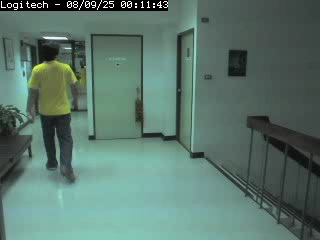
\includegraphics[width=2.5in]{figures/shadow-example.png}
%   \caption[Self and cast shadow in a real-world scene image]{Self and
%   cast shadow in a real-world scene image. Self shadow is on the back
%   of the person and cast shadow in on the ground.}
%  \label{fig:shadow-example}
%  \end{center}
%\end{figure}
%
%Removing shadows can significantly improve the performance of the
%computer vision tasks such as tracking, segmentation, and object
%detection. Since the detection and tracking is the core of video
%surveillance systems, poor detection and tracking can cause the
%problems to the next processing step such as feature extraction and
%behavior modeling. Background modeling techniques alone cannot solve
%the problems. We need an algorithm to detect and remove shadows.
%Therefore, in this dissertation, we explore and develop the shadow
%detection and removal algorithms. The experiments analyze the
%algorithms on the real-world video data.
%
%For the existing shadow detection
%methods, \shortciteA{cucchiara01shadow} and \shortciteA{chen08shadow}
%use the HSV color information to distinguish shadows from moving
%objects. Their approach is based on the assumption that only the
%intensity of the area covered by shadows will significantly change.
%Therefore, they can detect shadows using the following equation.
%\[
%  SP_t (x,y) = \left\{ \begin{array}{l}
%  1\;\;\;{\rm if}\;\alpha  \le \frac{{I_t^V (x,y)}}{{B_t^V (x,y)}} \le \beta\\ 
%  \quad \quad  \wedge (I_t^S (x,y) - B_t^S (x,y)) \le T_S  \\ 
%  \quad \quad  \wedge \left| {I_t^H (x,y) - B_t^H (x,y)} \right| \le T_H\\ \\
%  0\;\;\;{\rm otherwise}, \\ 
%  \end{array} \right.
%\]
%where $SP_t(x,y)$ is the binary mask of shadows at pixel $(x,y)$ at
%time $t$.  $I_t^H$, $I_t^S$, $I_t^V$, $B_t^H$, $B_t^S$, and $B_t^V$
%are H, S, V components of foreground pixel $I_t(x,y)$ and background
%pixel $B_t(x, y)$ at pixel $(x,y)$ at time $t$, respectively. They
%prevent the foreground pixel being classified into shadows by setting
%two thresholds $\alpha$ and $\beta$.  The parameter $\beta$ is set
%under 1 and $\alpha$ is set over 0. $T_S$ and $T_H$ are discovered by
%experiments.
%
%\shortciteA{tian05shadow}, \shortciteA{jacques05shadow},
%and \shortciteA{tan06shadow} apply the normalized cross-correlation
%(NCC) to detect shadows based on the assumption that the intensity of
%shadows is proportional to the incident light ,and shadow pixels are
%darker than background pixels, or it can be said that the shadows are
%the scaled versions of background. Therefore, using the NCC, they can
%identify the scaled versions of the same signal. They perform the NCC
%on the foreground mask from the background subtraction progress. For
%each pixel $(i, j)$ of the foreground mask, they considered a $(2N +
%1) \times (2N + 1)$ template $T_{ij}$, and defined $T_{ij}(n, m) =
%I(i+n, j+m)$ for $-N \le n \le N$, $-N \le m \le N$. $B(i,j)$ is the
%background image formed by temporal median filtering. The NCC at pixel
%$(x,y)$ is defined as.
%\[
%  NCC(i,j) = \frac{{ER(i,j)}}{{E_B (i,j)E_{T_{ij} } }},
%\]
%where
%\[
%  ER(i,j) = \sum\limits_{n = -N}^N {\sum\limits_{m = -N}^N {B(i + n,j
%  + m)T_{ij} (n,m)} },
%\]
%\[
%  E_B (i,j) = \sqrt {\sum\limits_{n = -qN}^N {\sum\limits_{m = -N}^N
%  {B(i + n,j + m)^2 } } },
%\]
%\[
%  E_{T_{ij} } = \sqrt {\sum\limits_{n = -N}^N {\sum\limits_{m = -N}^N
%  {T_{ij} (n,m)^2 } } }.
%\]
%For a pixel in a shadow region, the NCC value should be large (close
%to one) and the $E_{T_{ij}}$ of this region should be lower than the
%$E_B (i,j)$.  Consequently, a pixel is classified into shadow if
%\[
%  NCC(i,j) \ge L_{NCC} 
%\]
%and
%\[
%  E_{T_{ij} } < E_B (i,j),
%\]
%where $L_{NCC}$ is a threshold. Figure \ref{fig:tian-shadow-result}
%shows some examples of the results from the work
%of \shortciteA{tian05shadow}.
%
%\begin{figure}
%  \centering
%  \begin{tabular}{c}
%    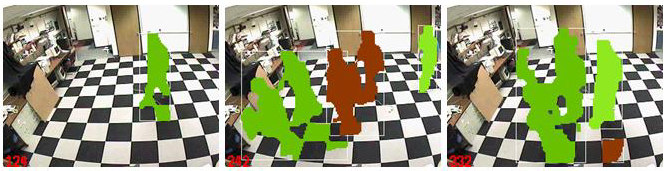
\includegraphics[scale=0.7]{figures/tian-mog-results.png}\\
%    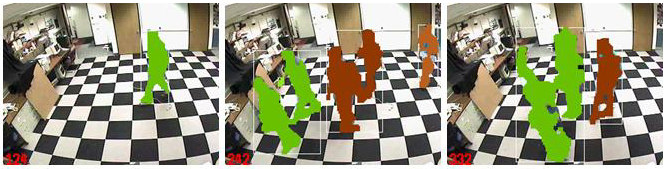
\includegraphics[scale=0.7]{figures/tian-shadow-results.png}
%  \end{tabular}
%  \caption[Examples of the background subtraction and shadow removal
%  results.]{Examples of the background subtraction and shadow removal
%  results. Upper row shows the results of the MoG background modeling
%  and lower row shows the results from the work of Tian et
%  al. Reprinted from the work of Tian et al.\ (2005).}
%  \label{fig:tian-shadow-result}
%\end{figure}
%
%Some authors found that the blue color component increases while the
%red color component decreases in a shadow
%region. \shortciteA{mikic00shadow} combine this information and
%normalized the blue and red color components as one of their
%features. After that, they apply a probabilistic model to classify
%shadow pixels in traffic scenes. They also assume that the background
%and shadow values follow a Gaussian distribution, and assume the
%foreground values follow an uniform distribution. They iteratively
%estimate the posterior probabilities of the pixel belonging to each
%of the three classes: background, shadow, and foreground until one of
%the probabilities reaches a fixed threshold. The pixel is then
%classified into one of those classes. If none of the three
%probabilities reaches the threshold, the pixel will be classified as
%background.
%
%\shortciteA{xu05shadow} assume that the chromaticity in a shadow
%region should be the same as when it is illuminated. Based on the
%information, they use a normalized chromatic color space to remove
%shadows. In this paper, they normalize the red and green color
%components. Then they define a set of thresholds for brightness and
%color distortion to classify a pixel value into foreground, highlight,
%or shadow.
%
%\shortciteA{hong03background} mention that there are both
%chromaticity and brightness in each pixel value in the RGB space. They
%remove the lightness by using the normalized RGB color space since the
%normalized RGB color space contains only the chromaticity. Thus, they
%use this information to propose their background subtraction
%approach. \shortciteA{havasi06geometric} illustrate that the color
%based method works well in case of weak shadow, but strong
%shadow. Hence, they integrate the geometric information into the
%detection process and came up with an iterative Bayesian framework
%which combines both the color and geometric information to improve the
%detection results.
%
%\section{Methodology}
%
%We use NCC and the maximum likelihood based on the HSV color
%information extracted from a set of training images to remove shadows.
%
%We compute the difference of hue $H_{\text{diff}}$, saturation
%$S_{\text{diff}}$, and value $V_{\text{diff}}$ components under the
%mask between the current and background frames. We simply calculate
%the probability as follows.
%
%\begin{equation*}
%  \begin{array}{ccl}
%    P(M_{\text{xy}} \mid A_{\text{xy}} = \text{sh}) 
%            & = & P(H_{\text{diff}}^{\text{sh}} \mid A_{\text{xy}} = \text{sh})
%                  P(S_{\text{diff}}^{\text{sh}} \mid A_{\text{xy}} = \text{sh}) \\
%            &   & P(V_{\text{diff}}^{\text{sh}} \mid A_{\text{xy}} = \text{sh}),
%  \end{array}
%\end{equation*}
%where $M_{xy}$ is a measurement at pixel $(x,y)$. To make the problem
%simple, we assume that the distribution of the difference of hue,
%saturation, and value components follows a normal distribution as
%follows.
%\begin{equation*}
%  P(H_{\text{diff}}^{\text{sh}} \mid A_{\text{xy}} = \text{sh}) \sim {\cal
%    N}(H_{\text{diff}}^{\text{sh}} ; 0, \sigma^2_{h_{\text{diff}}^{\text{sh}}}),
%\end{equation*}
%
%\begin{equation*}
%  P(S_{\text{diff}}^{\text{sh}} \mid A_{\text{xy}} = \text{sh}) \sim {\cal
%    N}(S_{\text{diff}}^{\text{sh}} ; 0, \sigma^2_{s_{\text{diff}}^{\text{sh}}}),
%\end{equation*}
%and
%\begin{equation*}
%  P(V_{\text{diff}}^{\text{sh}} \mid A_{\text{xy}} = \text{sh}) \sim {\cal
%    N}(V_{\text{diff}}^{\text{sh}} ; 0, \sigma^2_{v_{\text{diff}}^{\text{sh}}}).
%\end{equation*}
%
%\noindent Similarly, the measurement given the foreground assignment
%can be computed as follows.
%
%\begin{equation*}
%  \begin{array}{ccl}
%    P(M_{\text{xy}} \mid A_{\text{xy}} = \text{fg}) 
%            & = & P(H_{\text{diff}}^{\text{fg}} \mid A_{\text{xy}} = \text{fg})
%                  P(S_{\text{diff}}^{\text{fg}} \mid A_{\text{xy}} = \text{fg}) \\
%            &   & P(V_{\text{diff}}^{\text{fg}} \mid A_{\text{xy}} = \text{fg})
%  \end{array}
%\end{equation*}
%
%\noindent Each component is defined as follows.
%
%\begin{equation*}
%  P(H_{\text{diff}}^{\text{fg}} \mid A_{\text{xy}} = \text{fg}) \sim {\cal
%    N}(H_{\text{diff}}^{\text{fg}} ; 0, \sigma^2_{h_{\text{diff}}^{\text{fg}}}),
%\end{equation*}
%
%\begin{equation*}
%  P(S_{\text{diff}}^{\text{fg}} \mid A_{\text{xy}} = \text{fg}) \sim {\cal
%    N}(S_{\text{diff}}^{\text{fg}} ; 0, \sigma^2_{s_{\text{diff}}^{\text{fg}}}),
%\end{equation*}
%and
%\begin{equation*}
%  P(V_{\text{diff}}^{\text{fg}} \mid A_{\text{xy}} = \text{fg}) \sim {\cal
%    N}(V_{\text{diff}}^{\text{fg}} ; 0, \sigma^2_{v_{\text{diff}}^{\text{fg}}}).
%\end{equation*}
%
%Finally, we use the maximum likelihood approach to classify a pixel
%whether it is foreground or shadow.
%
%\section{Experimental Results}
%
%To collect data, we used ZoneMinder \shortcite{zoneminder} to capture
%video during two weeks. We set up a machine with a Web camera on the
%second floor in the Computer Science and Information Management (CSIM)
%building to capture activities in the scene.
%
%We have experimented with a shadow detection method using normalized
%cross correlation (NCC).  We compute the grayscale correlation between
%the foreground pixels and a background image constructed as the mean
%over each mixture of Gaussian distribution. Any foreground pixels
%whose NCC with the background are above some threshold
%$L_{\text{NCC}}$ are removed. In the experiments, we set
%$L_{\text{NCC}} = 0.995$. The results are shown in
%Figure \ref{fig:shadow-outdoor-result}. NCC works well in the outdoor
%scenes with visible background texture inside shadows. However, when
%we applied it in the indoor scenes, it does not work very well in many
%cases due to the lighting effect as shown in
%Figure \ref{fig:shadow-poor-result}.
%
%\begin{figure}[t]
%  \centering
%  \begin{tabular}{ccc}
%    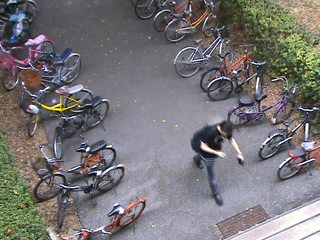
\includegraphics[width=0.28\linewidth]{figures/shadow-result01.png} &
%    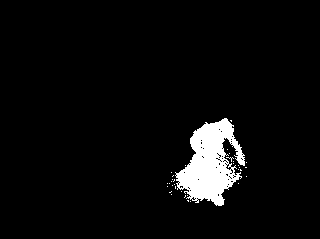
\includegraphics[width=0.28\linewidth]{figures/shadow-result02.png} &
%    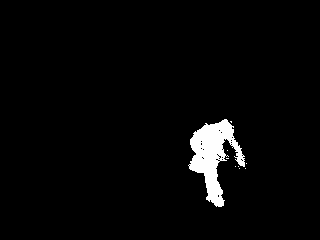
\includegraphics[width=0.28\linewidth]{figures/shadow-result03.png}
%    \\
%    (a) & (b) & (c)
%    \end{tabular}
%  \caption{Sample foreground extraction and shadow removal results in
%    an outdoor scene.  (a) Original image. (b) Foreground pixels
%    according to background model.  (c) Foreground pixels after shadow
%    removal.}
%  \label{fig:shadow-outdoor-result}
%\end{figure}
%
%\begin{figure}[t]
%  \centering
%  \begin{tabular}{ccc}
%    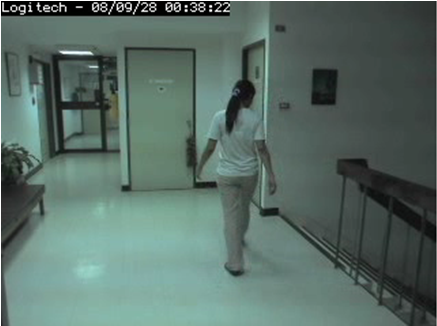
\includegraphics[width=0.28\linewidth]{figures/shadow-poor-result01.png} &
%    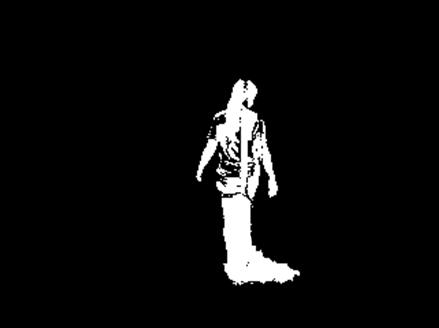
\includegraphics[width=0.28\linewidth]{figures/shadow-poor-result02.png} &
%    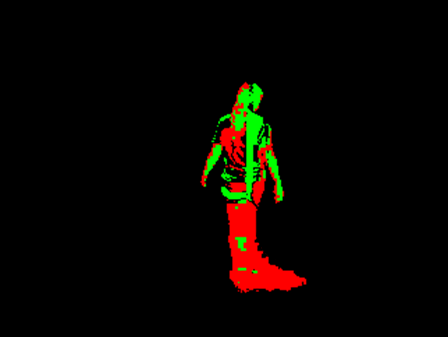
\includegraphics[width=0.28\linewidth]{figures/shadow-poor-result03.png}
%    \\
%    (a) & (b) & (c)
%  \end{tabular}
%  \caption{Sample poor shadow removal results in an indoor scene.  (a)
%    Original image. (b) Foreground pixels according to background
%    model.  (c) Foreground pixels after shadow removal. Red pixels
%    show the positives, and green pixels show the negatives.}
%  \label{fig:shadow-poor-result}
%\end{figure}
%
%We have performed another experiment using a maximum likelihood
%approach on the HSV color space. We first compute the difference of
%hue, saturation, and value under the mask of the current and
%background frames from a set of training images. The distributions of
%those values under the foreground mask are shown in
%Figure \ref{fig:foreground-distribution}, and the distributions under
%the shadow mask are shown in Figure
%\ref{fig:shadow-distribution}. For the hue and saturation values, we
%subtracted the current frame by the background frame, but for the
%intensity value, to get the positive values, we subtracted the
%background frame by the current frame.
%
%\begin{figure}[t]
%  \centering
%  \subfloat[]{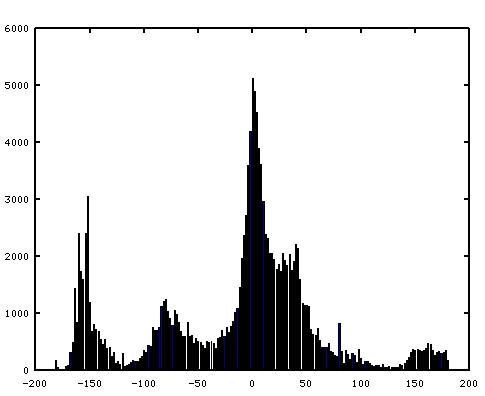
\includegraphics[width=0.32\linewidth]{figures/foreground_diff_h.png}}
%  \hspace{0.05in}
%  \subfloat[]{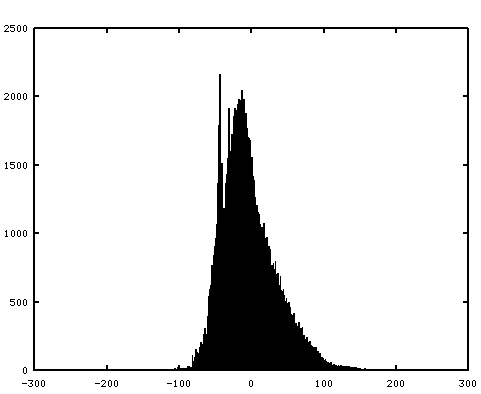
\includegraphics[width=0.32\linewidth]{figures/foreground_diff_s.png}}
%  \hspace{0.05in}
%  \subfloat[]{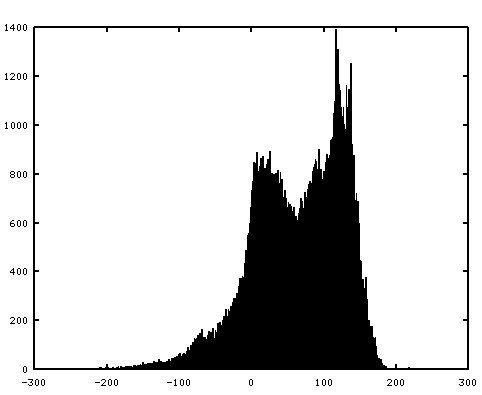
\includegraphics[width=0.32\linewidth]{figures/foreground_diff_v.png}}
%  \caption{Distribution of the difference of hue, saturation, and
%    value under the foreground mask. (a) Difference of hue.(b)
%    Difference of saturation. (c) Difference of value.}
%  \label{fig:foreground-distribution}
%\end{figure}
%
%\begin{figure}[t]
%  \centering
%  \subfloat[]{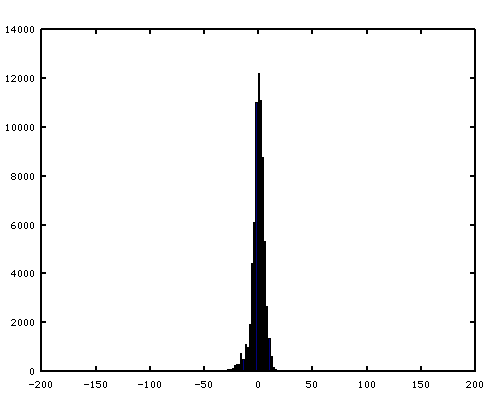
\includegraphics[width=0.32\linewidth]{figures/shadow_diff_h.png}}
%  \hspace{0.05in}
%  \subfloat[]{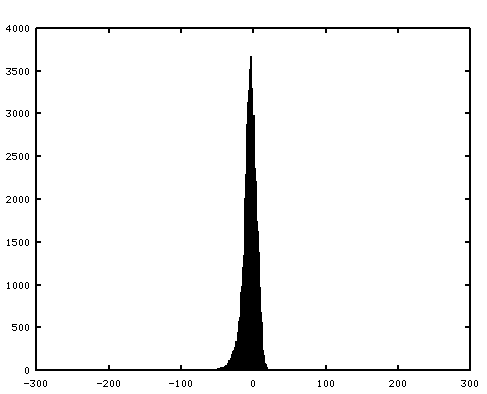
\includegraphics[width=0.32\linewidth]{figures/shadow_diff_s.png}}
%  \hspace{0.05in}
%  \subfloat[]{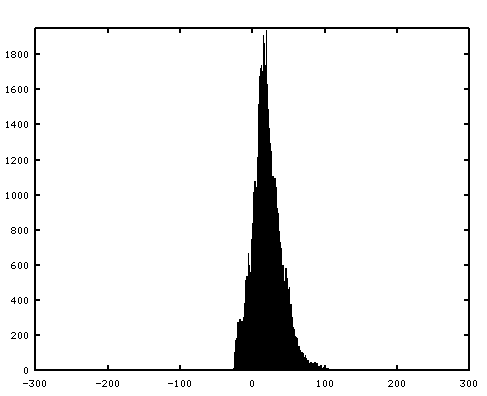
\includegraphics[width=0.32\linewidth]{figures/shadow_diff_v.png}}
%  \caption{Distribution of the difference of hue, saturation, and
%    value under the shadow mask. (a) Difference of hue. (b) Difference
%    of saturation. (c) Difference of value.}
%  \label{fig:shadow-distribution}
%\end{figure}
%
%The results for the maximum likelihood approach compared to the NCC
%approach are shown in Figure \ref{fig:comparison-shadow-results}.
%
%\begin{figure}[t]
%  \centering
%  \begin{tabular}{cccc}
%    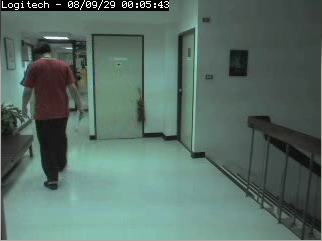
\includegraphics[width=0.22\linewidth]{figures/shadow-original.png} &
%    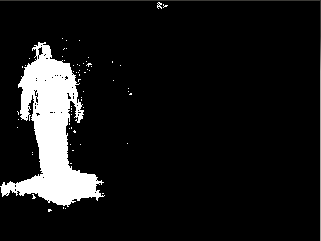
\includegraphics[width=0.22\linewidth]{figures/shadow-bg-results.png} &
%    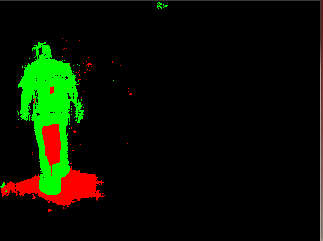
\includegraphics[width=0.22\linewidth]{figures/shadow-ncc-results.png} &
%    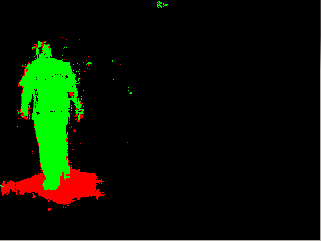
\includegraphics[width=0.22\linewidth]{figures/shadow-ml-results.png}
%    \\
%    (a) & (b) & (c) & (d)
%    \end{tabular}
%  \caption{Shadow removal results in an indoor scene.  (a) Original
%    image. (b) Foreground pixels according to background model. (c)
%    Shadow detection using NCC.  (d) Shadow detection using the
%    maximum likelihood approach.}
%  \label{fig:comparison-shadow-results}
%\end{figure}
%








